
\documentclass[../open-optimization/open-optimization.tex]{subfiles}

%%%%%%%%%
\begin{document}
%%%%%%%%%

\titlepic{
	\begin{center}
	\begin{tabular}{ccccc}
	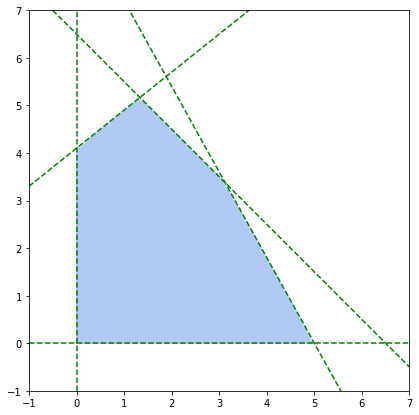
\includegraphics[scale = 0.3]{LP-feasible-region}  & \quad & 
	 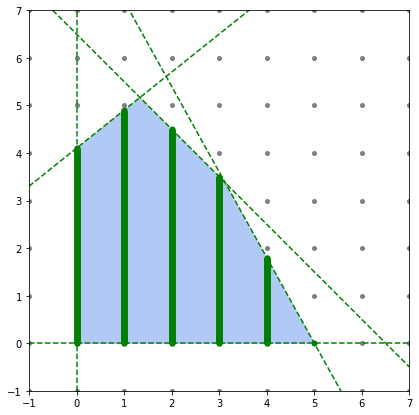
\includegraphics[scale = 0.3]{MIP-feasible-region} & \quad &
	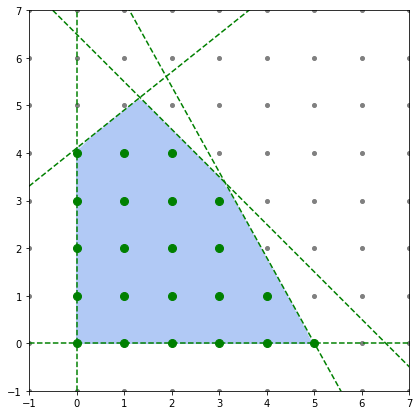
\includegraphics[scale = 0.3]{IP-feasible-region}%% \\
	%% LP && MIP && IP\\
	%% \\
	%% $Ax \leq b$ & &$Ax \leq b$ && $Ax \leq b$\\
	%% & &$x_1 \in \Z$ & &$x_1, x_2 \in \Z$
	\end{tabular}
	\end{center}\nopagebreak
        \begin{center}
          
\includegraphics[width=\linewidth]{../../../open-optimization-common/logos/logo-open-optimization-oer-wide}
        \end{center}
}
\maketitle
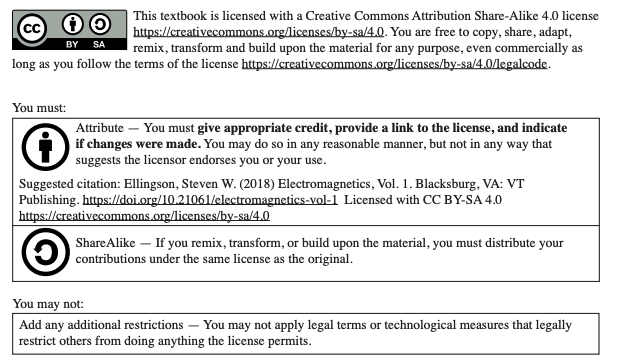
\includegraphics[scale = 0.65]{creative-commons-statement}


This work is done in alignment with the mission of UNESCO Open Educational Resources \url{https://en.unesco.org/themes/building-knowledge-societies/oer}
\begin{center}
\includegraphics[scale = 0.1]{Global_Open_Educational_Resources_Logo.svg}\footnotemark
\end{center}
\footnotetext{\url{https://en.wikipedia.org/wiki/Open_educational_resources\#/media/File:Global_Open_Educational_Resources_Logo.svg}}

The source code of this book is available from
\url{https://github.com/open-optimization/}

\newpage

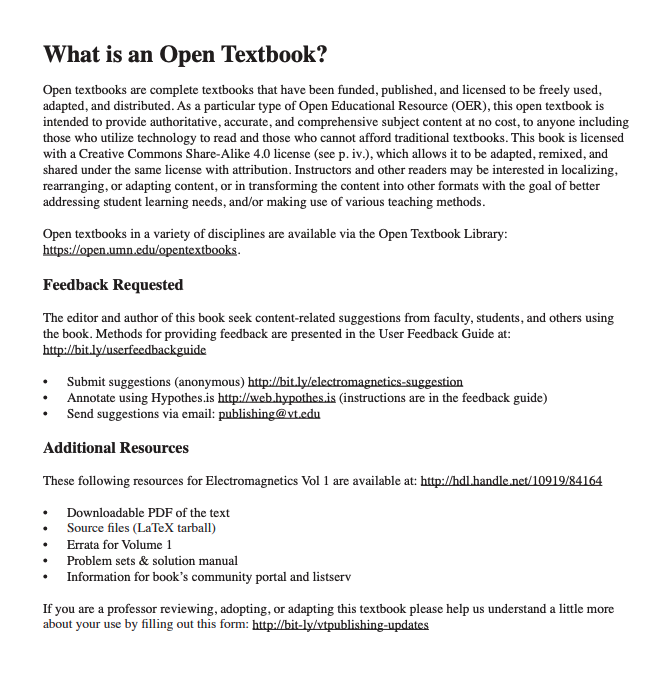
\includegraphics[scale = 0.65]{what-is-open-textbook}\footnotemark
\footnotetext{Take from open-source electromagnetics book}

\newpage

\section*{Preface}
%% FIXME: Convert this to latex by pandoc, include the .tex file
\verbatiminput{../../../open-optimization-common/README-open-optimization.md}

%%%%%%%%%
\end{document}
%%%%%%%%%
%%% Local Variables:
%%% mode: latex
%%% TeX-master: "../open-optimization/open-optimization"
%%% End:
